\documentclass[aspectratio=169,10pt]{beamer}
\usepackage{../common/beamer_theme_bio}

\title{\textbf{Biostatistiques Appliquées}}
\subtitle{Chapitre VII : Interprétation d'une Analyse Expérimentale, Bonnes Pratiques \& Éthique}
\author{\textbf{Dr. Sarra BENMOUMOU (Ph.D.)}}
\institute{
  Faculté des Sciences --- Département de Biologie\\
  Master 2 : Biochimie Appliquée\\
  \textbf{Université M'Hamed Bougara de Boumerdès (UMBB)}
}
\date{Année Universitaire 2024 -- 2025}

\begin{document}

% --------------------------------------------------------
\begin{frame}[plain]
  \titlepage
\end{frame}

% --------------------------------------------------------
\begin{frame}{Plan Détaillé du Chapitre VII}
  \tableofcontents
\end{frame}

% ========================================================
\section{Conception Expérimentale \& Plan d'Expérience (DoE)}
% ========================================================

\begin{frame}{Les Trois Piliers Fondamentaux du Plan d'Expérience (DoE)}
  \begin{columns}[onlytextwidth, T]
    \begin{column}{0.31\linewidth}
      \begin{conceptbox}{1. Randomisation}
        \footnotesize
        \textbf{Principe :} Attribuer les unités expérimentales (rats, puits, souris) aux traitements de façon strictement aléatoire.
        \vspace{1mm}
        \par \textbf{Objectif :} Neutraliser les facteurs de confusion cachés (effet d'emplacement de la cage, gradient thermique dans l'étuve).
      \end{conceptbox}
    \end{column}
    \begin{column}{0.31\linewidth}
      \begin{conceptbox}{2. Vraie Réplication}
        \footnotesize
        \textbf{Principe :} Multiplier les véritables unités biologiques indépendantes ($N$).
        \vspace{1mm}
        \par \textbf{Objectif :} Mesurer la variabilité inter-individuelle biologique réelle sans la confondre avec l'erreur instrumentale de pipetage.
      \end{conceptbox}
    \end{column}
    \begin{column}{0.31\linewidth}
      \begin{conceptbox}{3. Contrôle Local (Blocs)}
        \footnotesize
        \textbf{Principe :} Regrouper les essais par « blocs » homogènes (même jour de manipulation, même kit ELISA).
        \vspace{1mm}
        \par \textbf{Objectif :} Absorber la variance liée aux conditions extérieures sans affaiblir la comparaison des traitements.
      \end{conceptbox}
    \end{column}
  \end{columns}
\end{frame}

\begin{frame}{Le Piège Majeur : Réplicat Biologique vs Pseudoréplication}
  \begin{columns}[onlytextwidth, T]
    \begin{column}{0.48\linewidth}
      \begin{conceptbox}{Vrai Réplicat Biologique ($N$)}
        \begin{itemize}
          \item Échantillons issus d'animaux, de donneurs ou de cultures cellulaires \textbf{indépendants}.
          \item Représente la variabilité naturelle de la population cible.
          \item \textbf{C'est la seule unité valide} pour les degrés de liberté ($df = N - k$) d'un test statistique (Student, ANOVA).
        \end{itemize}
      \end{conceptbox}
    \end{column}
    \begin{column}{0.48\linewidth}
      \begin{warnbox}{Pseudoréplication Technique ($n$)}
        \begin{itemize}
          \item Mesures répétées (triplicats) sur \textbf{un même extrait biologique} ou le même animal.
          \item Évalue uniquement la précision du pipetage ou du spectrophotomètre.
          \item \textbf{Erreur grave :} Traiter $3 \times 3 = 9$ puits comme $N=9$ au lieu de faire la moyenne par animal ($N=3$). Ceci gonfle artificiellement les $df$ et génère des faux positifs massifs !
        \end{itemize}
      \end{warnbox}
    \end{column}
  \end{columns}
\end{frame}

\begin{frame}{Puissance Statistique ($1-\beta$) \& Détermination d'Effectif ($N$)}
  \begin{columns}[onlytextwidth, T]
    \begin{column}{0.50\linewidth}
      \begin{center}
        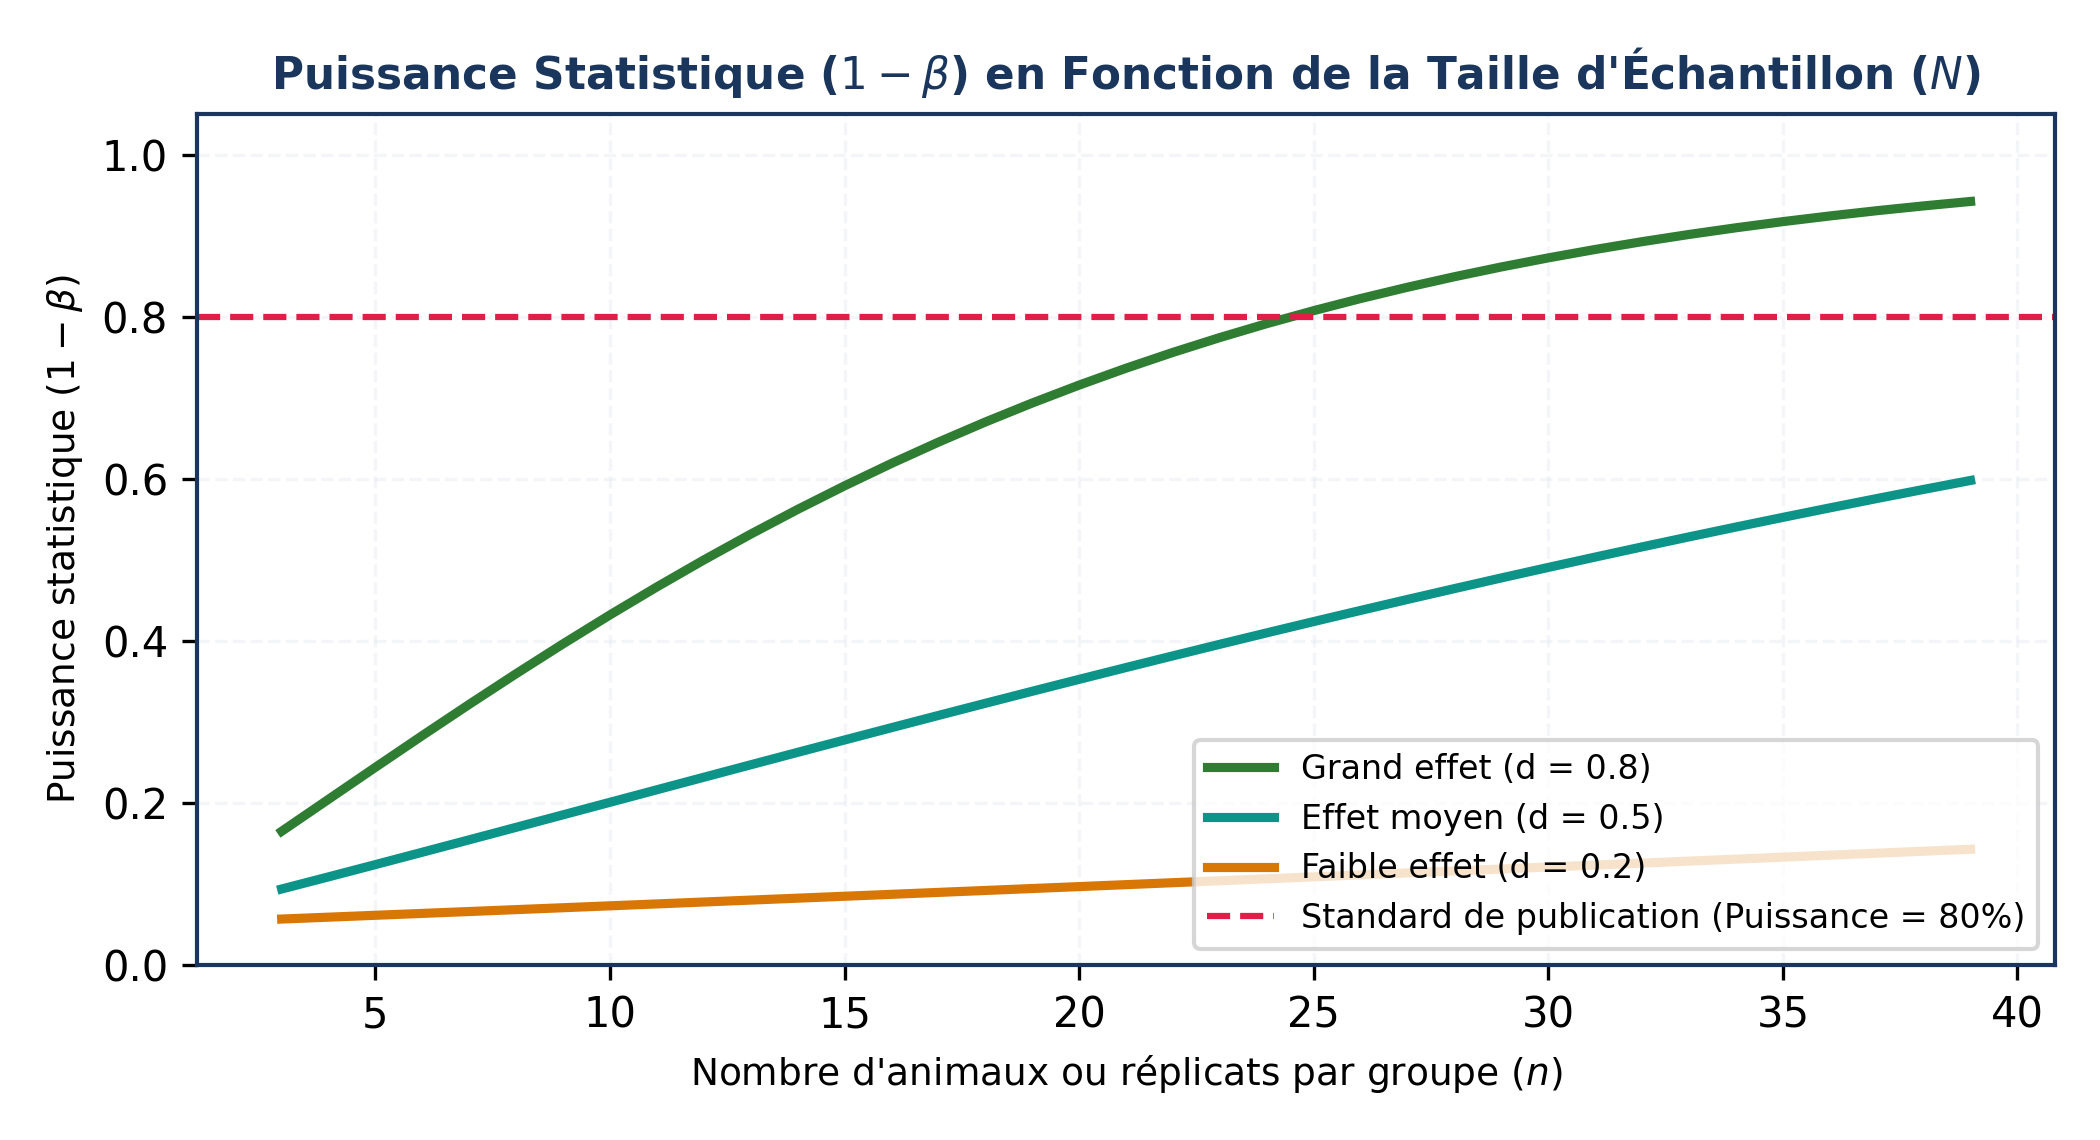
\includegraphics[width=\linewidth, keepaspectratio]{../figures/fig07_power_sample_size_curve.png}
      \end{center}
    \end{column}
    \begin{column}{0.48\linewidth}
      \begin{conceptbox}{Calcul d'Effectif A Priori}
        \footnotesize
        Fixer la taille d'échantillon \textbf{avant} l'essai :
        \begin{equation*}
          N = f(\alpha = 0.05, \, 1-\beta \ge 0.80, \, d)
        \end{equation*}
        Pour un effet moyen ($d=0.5$), il faut au moins $n \ge 17$ animaux/groupe !
      \end{conceptbox}
      \vspace{1mm}
      \begin{warnbox}{Le Drame du Sous-Effectif ($n=3$)}
        \footnotesize
        Tester $n=3$ rats conduit à une puissance $< 25\%$ :
        \begin{itemize}
          \item Faux négatif garanti pour un effet modéré.
          \item Biais d'exagération si $p < 0.05$ par chance.
        \end{itemize}
      \end{warnbox}
    \end{column}
  \end{columns}
\end{frame}

% ========================================================
\section{La Crise de Reproductibilité \& Les Pratiques Douteuses}
% ========================================================

\begin{frame}{Les Fléaux Méthodologiques : $p$-hacking, HARKing \& Arrêt Précoce}
  \begin{table}[h]
    \centering
    \small
    \resizebox{\linewidth}{!}{%
    \begin{tabular}{lp{6.2cm}p{6.8cm}}
      \toprule
      \textbf{Pratique Déviante} & \textbf{Mécanisme \& Réalité Expérimentale} & \textbf{Conséquence Biologique} \\
      \midrule
      \textbf{$p$-hacking} & Tester plusieurs tests statistiques, supprimer des outliers arbitrairement ou ajouter des covariables jusqu'à ce que $p < 0.05$. & Découverte de biomarqueurs fantômes non reproductibles par les autres laboratoires. \\
      \addlinespace
      \textbf{HARKing} & Formuler l'hypothèse de recherche \textit{a posteriori}, après avoir inspecté visuellement les données significatives. & Présentation d'une fluctuation aléatoire fortuite comme une découverte physiologique majeure. \\
      \addlinespace
      \textbf{Arrêt Précoce} & Tester la significativité après chaque rat manipulé et arrêter l'expérience dès que $p$ franchit le seuil de $0.05$. & Inflation incontrôlée de l'erreur de type I (le risque $\alpha$ réel peut atteindre 30\% au lieu de 5\%). \\
      \bottomrule
    \end{tabular}%
    }
  \end{table}
  \vspace{1mm}
  \begin{takeawaybox}{Principe d'Intégrité Scientifique}
    Les hypothèses, le plan d'analyse statistique et les critères d'exclusion des valeurs aberrantes doivent être \textbf{fixés avant l'acquisition des données} (idéalement pré-enregistrés).
  \end{takeawaybox}
\end{frame}

\begin{frame}{Transparence Graphique : Pourquoi Bannir les Barplots « Dynamite »}
  \begin{columns}[onlytextwidth, T]
    \begin{column}{0.50\linewidth}
      \begin{center}
        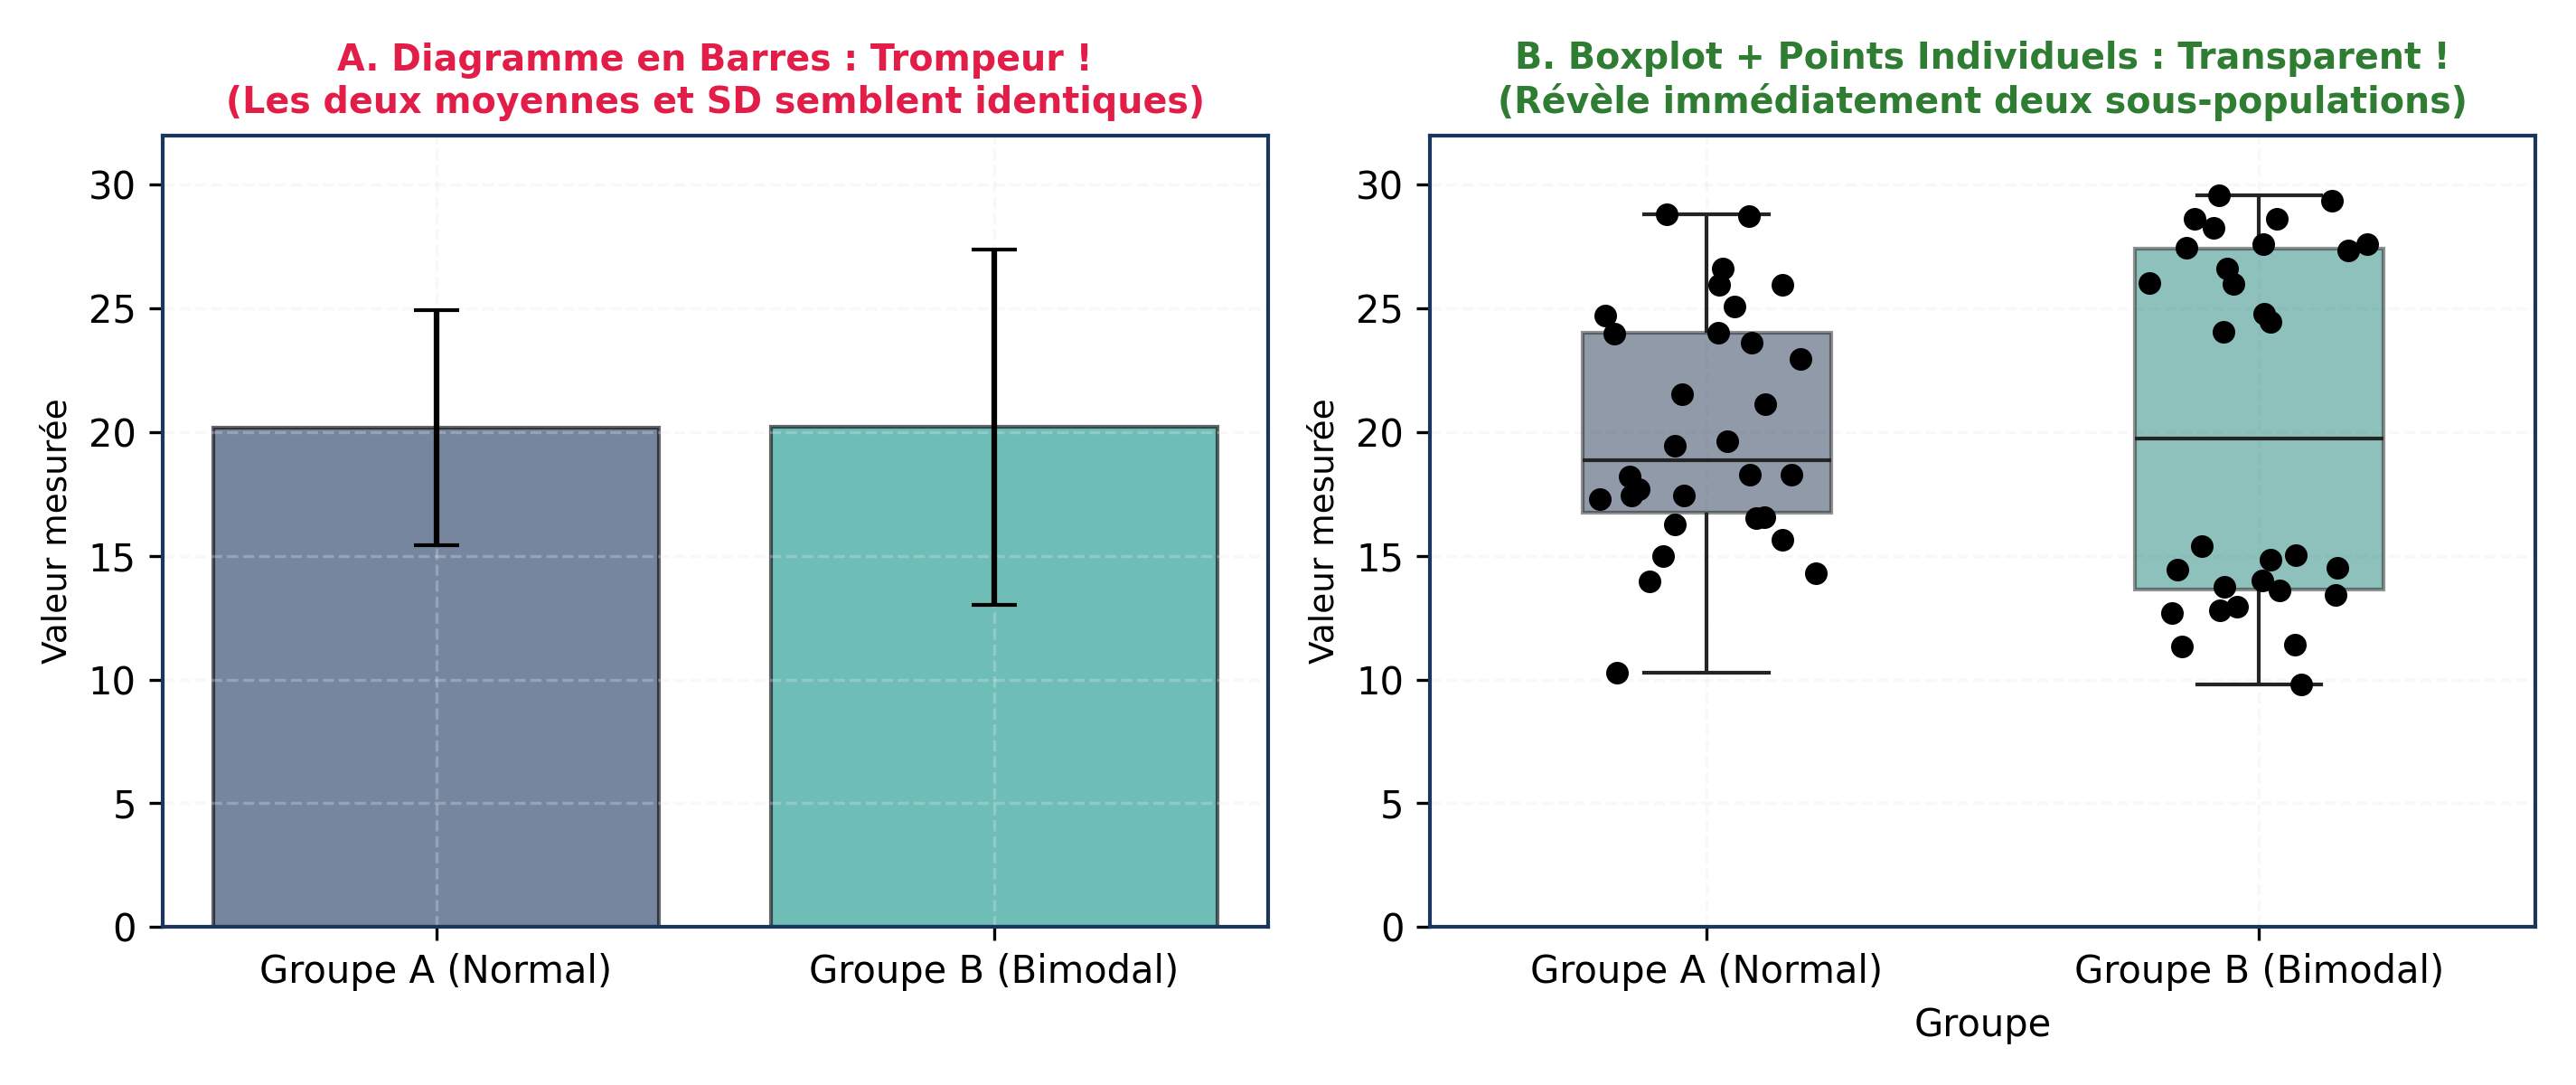
\includegraphics[width=\linewidth, keepaspectratio]{../figures/fig07_barplot_vs_boxplot_transparency.png}
      \end{center}
    \end{column}
    \begin{column}{0.48\linewidth}
      \begin{warnbox}{Le Défaut des Barres Pleines}
        \footnotesize
        Une barre pleine avec barre d'erreur dissimule la structure des données. Elle masque les distributions bimodales, l'asymétrie et les outliers majeurs.
      \end{warnbox}
      \vspace{1mm}
      \begin{conceptbox}{Le Standard Moderne de Publication}
        \footnotesize
        Privilégier les \textbf{Boxplots} ou \textbf{Violin plots} avec \textbf{superposition de tous les points réels} (Scatter/Jitter). Exigé par \textit{Nature}, \textit{Cell} et \textit{PLOS Biology}.
      \end{conceptbox}
    \end{column}
  \end{columns}
\end{frame}

% ========================================================
\section{Standards Internationaux de Publication Scientifique}
% ========================================================

\begin{frame}{Directives Internationales : Guides SAMPL \& ARRIVE 2.0}
  \begin{columns}[onlytextwidth, T]
    \begin{column}{0.48\linewidth}
      \begin{conceptbox}{Guide SAMPL (Biostatistiques)}
        \footnotesize
        \textbf{Statistical Analyses and Methods in the Published Literature} :
        \begin{itemize}
          \item Indiquer le test exact utilisé pour chaque comparaison.
          \item Préciser si les conditions de validité (normalité, variance) ont été vérifiées et par quel test.
          \item Toujours associer aux $p$-values les \textbf{tailles d'effet} et les \textbf{intervalles de confiance à 95\%} (IC 95\%).
          \item Indiquer la valeur exacte de $p$ (ex: $p = 0.024$ au lieu de $p < 0.05$ ou « NS »).
        \end{itemize}
      \end{conceptbox}
    \end{column}
    \begin{column}{0.48\linewidth}
      \begin{biobox}{Directives ARRIVE 2.0 (In Vivo \& In Vitro)}
        \footnotesize
        \textbf{Animal Research: Reporting of In Vivo Experiments} :
        \begin{itemize}
          \item Déclaration explicite du protocole de randomisation et de mise en aveugle (\textit{blind testing}).
          \item Justification du calcul de taille d'échantillon ($N$) selon le principe éthique des 3R (Remplacer, Réduire, Raffiner).
          \item Définition claire de l'unité expérimentale : l'animal individuel, la portée, ou le lot cellulaire.
        \end{itemize}
      \end{biobox}
    \end{column}
  \end{columns}
\end{frame}

\begin{frame}{Rdaction Modèle de la Section Biostatistique d'un Mémoire ou Article}
  \begin{tcolorbox}[colback=BioNavy!5, colframe=BioNavy, title={\faEdit\quad Modèle de Paragraphe pour la Section « Matériels \& Méthodes »}, width=\linewidth, boxrule=0.8pt, left=5pt, right=5pt]
    \footnotesize
    \textit{« Les données quantitatives sont exprimées sous forme de Moyenne $\pm$ Écart-Type ($SD$) pour $N$ réplicats biologiques indépendants. La normalité des distributions a été évaluée par le test de Shapiro-Wilk et l'égalité des variances par le test de Levene. Les comparaisons entre deux groupes ont été réalisées à l'aide d'un test $t$ de Student non apparié. Les cinétiques enzymatiques ont été modélisées par régression non linéaire directe selon l'équation de Michaelis-Menten via l'algorithme de Levenberg-Marquardt. Les effets croisés des traitements ont été évalués par ANOVA à deux facteurs suivie du test post-hoc de Tukey HSD pour ajuster le taux d'erreur de famille. Les analyses exploratoires multivariées ont été conduites par Analyse en Composantes Principales (ACP) et Classification Ascendante Hiérarchique (CAH, critère de Ward). Le seuil de significativité statistique a été fixé à $\alpha = 0.05$. L'ensemble des calculs a été réalisé sous Python (SciPy, Statsmodels, Scikit-learn). »}
  \end{tcolorbox}
\end{frame}

% ========================================================
\section{Arbre de Décision Intégratif \& Conclusion du Cours}
% ========================================================

\begin{frame}{Arbre de Décision : Quelle Méthode Choisir pour vos Données ?}
  \begin{center}
    \begin{tikzpicture}[scale=0.82, every node/.style={transform shape}]
      \node[draw=BioNavy, fill=BioNavy!10, rounded corners, minimum width=3cm, minimum height=0.9cm, align=center] (start) at (0,0) {\textbf{Nature de la}\\\textbf{Question Biologique}};
      
      \node[draw=BioTeal, fill=BioTeal!10, rounded corners, minimum width=3.2cm, minimum height=0.9cm, align=center] (m1) at (4.5, 1.8) {\textbf{Comparer des Moyennes}\\\tiny Différence entre lots};
      \node[draw=BioGreen, fill=BioGreen!10, rounded corners, minimum width=3.2cm, minimum height=0.9cm, align=center] (m2) at (4.5, 0) {\textbf{Modéliser une Relation}\\\tiny Dose-réponse, cinétique};
      \node[draw=BioNavy, fill=BioNavy!20, rounded corners, minimum width=3.2cm, minimum height=0.9cm, align=center] (m3) at (4.5, -1.8) {\textbf{Explorer la Structure}\\\tiny $p \gg n$, profils omiques};
      
      \node[draw=BioTeal, fill=white, rounded corners, minimum width=4cm, minimum height=0.8cm, align=center] (r1) at (10, 1.8) {\textbf{ANOVA Croisée ou Hiérarchisée}\\$+$ Post-hoc Tukey / Dunnett};
      \node[draw=BioGreen, fill=white, rounded corners, minimum width=4cm, minimum height=0.8cm, align=center] (r2) at (10, 0) {\textbf{Régression Linéaire (MCO)}\\ou \textbf{Non Linéaire (NLLS)}};
      \node[draw=BioNavy, fill=white, rounded corners, minimum width=4cm, minimum height=0.8cm, align=center] (r3) at (10, -1.8) {\textbf{ACP (Réduction dimension)}\\et \textbf{CAH (Classification)}};
      
      \draw[->, thick, BioNavy] (start) |- (m1);
      \draw[->, thick, BioNavy] (start) -- (m2);
      \draw[->, thick, BioNavy] (start) |- (m3);
      
      \draw[->, thick, BioTeal] (m1) -- (r1);
      \draw[->, thick, BioGreen] (m2) -- (r2);
      \draw[->, thick, BioNavy] (m3) -- (r3);
    \end{tikzpicture}
  \end{center}
\end{frame}

\begin{frame}[plain]
  \begin{center}
    \vspace{1.2cm}
    {\Huge\color{BioNavy}\textbf{Félicitations !}}\\[0.6cm]
    {\Large\textbf{Vous maîtrisez désormais les fondements de la Biostatistique Moderne}}\\[0.3cm]
    {\normalsize De la conception expérimentale rigoureuse à l'analyse de données omiques complexes,}\\[0.1cm]
    {\normalsize vous disposez de tous les atouts pour exceller dans vos recherches et votre carrière en biochimie.}\\[1.0cm]
    \textbf{Dr. Sarra BENMOUMOU (Ph.D.)}\\
    \small Département de Biologie --- Faculté des Sciences\\
    \textbf{Université M'Hamed Bougara de Boumerdès (UMBB)}
  \end{center}
\end{frame}

\end{document}
